\documentclass[UTF8]{article}
\usepackage{ctex,geometry,graphicx,float,makecell,rotating,multirow,diagbox}
\geometry{a4paper,scale=0.8}
\title{Homework\ 01}
\author{201850050\ 徐培宾}
\date{\today}

\begin{document}
    \maketitle
    \section{Q1:绘制saliency maps}
    \begin{figure}[H]
      \centering
      \includegraphics[width = 12cm]{./saliencymap/result/0_and_saliency_map.jpg}
      \\[5pt]
      \includegraphics[width = 12cm]{./saliencymap/result/1_and_saliency_map.jpg}
      \caption{saliency maps}
    \end{figure}
    A1:classifier容易在面部的五官上。
    \section{Q2:观察filter的output}
    \begin{figure}[H]
      \centering
      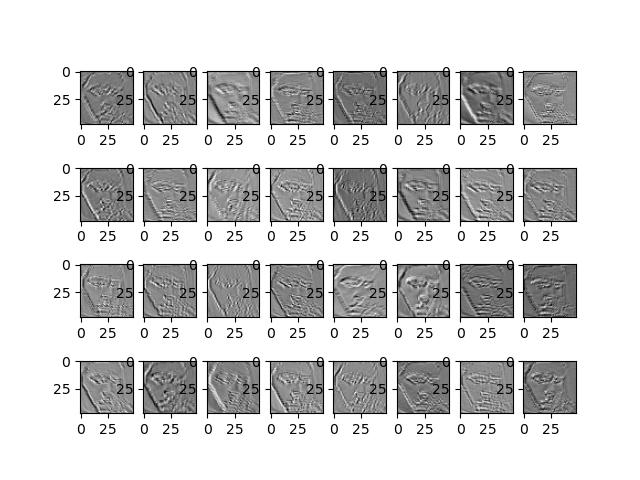
\includegraphics[width = 12cm]{./conv1.jpg}
      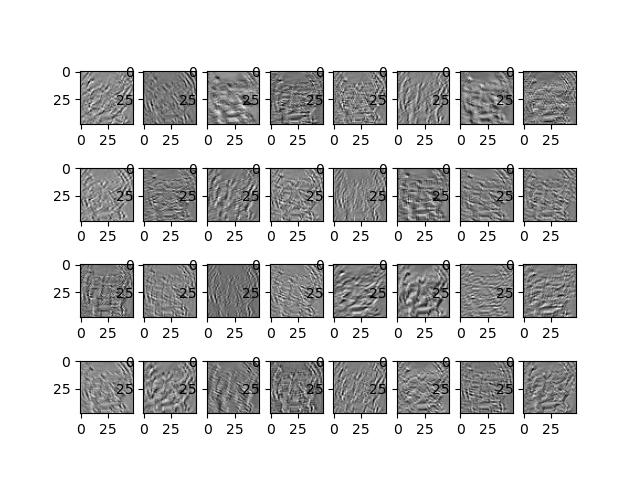
\includegraphics[width = 12cm]{./conv1-1.jpg}
      \caption{两张图片的Convlution1结果}
    \end{figure}
    A2:部分filter适合脸部轮廓清晰的图片,如filter7,15,22等,大部分filter能很好地提取所有纹理。
    \section{Q4:visualize\ CNN模型}
    \begin{figure}[H]
      \centering
      \includegraphics[width = 12cm]{./logs/test_accuracy.png}
      \\[18pt]
      \includegraphics[width = 12cm]{./logs/train_loss.png}
      \caption{模型训练的accuracy和EntropyLoss结果}
    \end{figure}
    \begin{figure}[H]
        \centering
        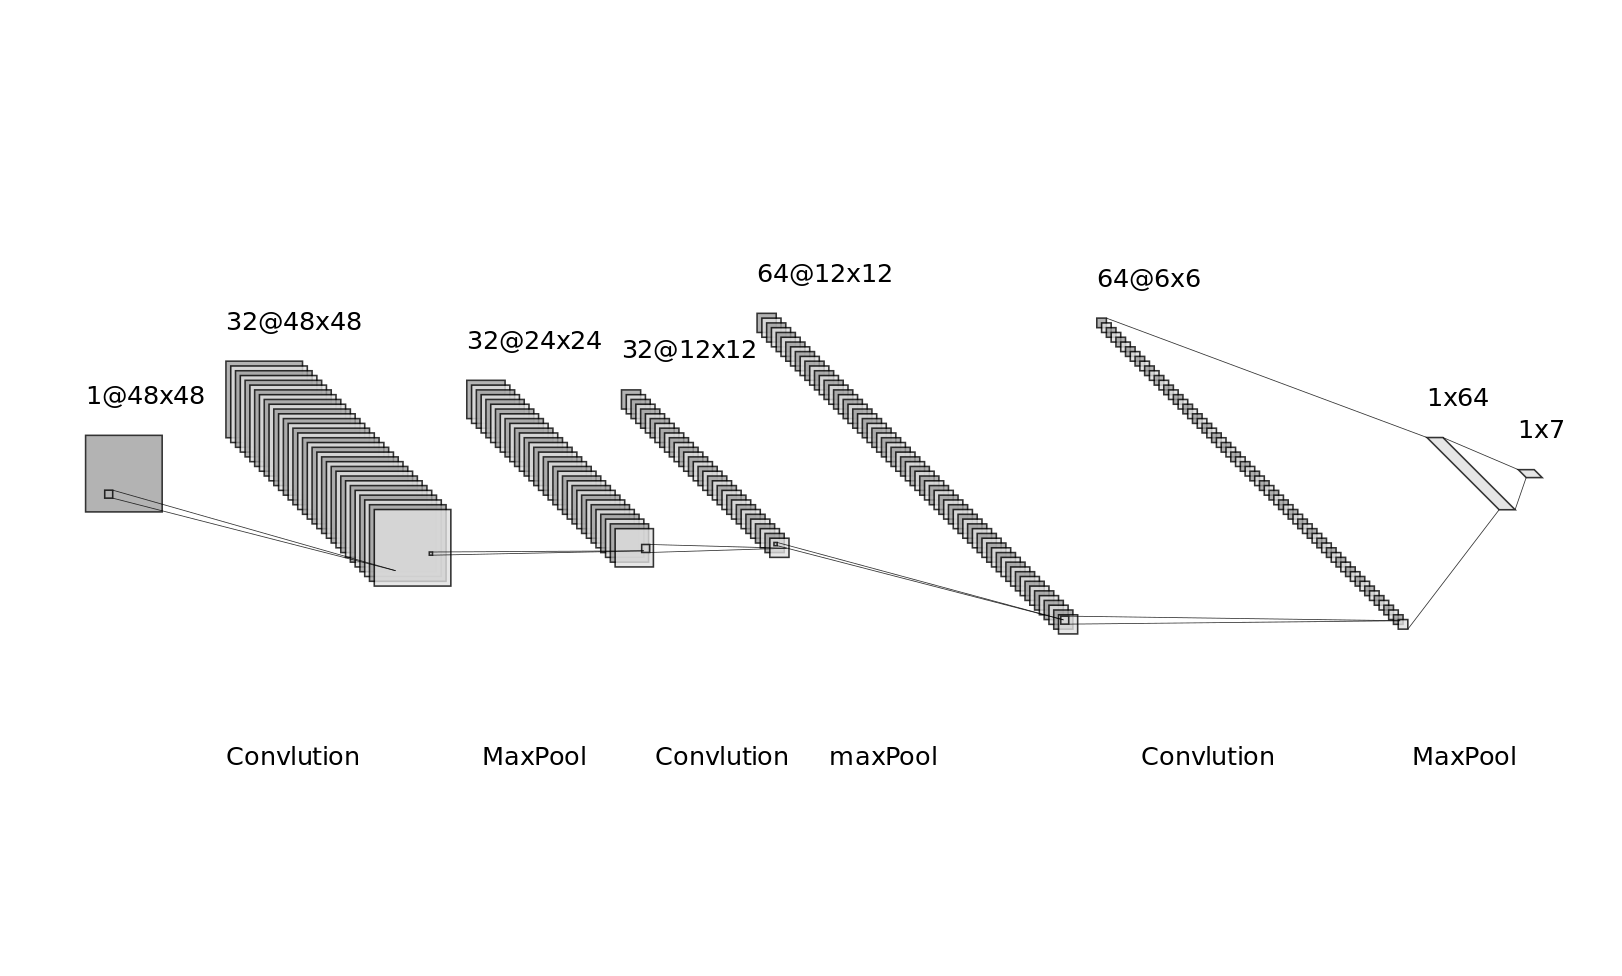
\includegraphics[width = 12cm]{./nn.png}
        \caption{模型的结构}
      \end{figure}
\end{document}    